\section{Injecting Pre-processed Features} 
\label{sec:feature}
To pursue better dialogue understanding and reasoning, different features either designed by experts back on linguistic knowledge or engineered with observations are proposed to simulate the human comprehension process.
Recognizing these features is not only independent dialogue analysis 
tasks but also critical enablers for downstream applications. 
A subset of these features has been proved helpful for dialogue summarization by extracting from $D$ explicitly and injecting it into the vanilla model.
We group different features into two sub-categories by their scopes:
\begin{itemize}
	\item \textbf{Intra-utterance features} are features within an utterance or for an individual utterance.
	\item \textbf{Inter-utterance features} are features connecting or distinguishing multiple utterances.
\end{itemize}



\subsection{Intra-Utterance Features}

We divide the intra-utterance features into three groups: word-level, 
phrase-level or utterance-level.


\subsubsection{Word-level}
Word-level intra-utterance features include TF-IDF weights, Part-of-speech (POS) tags, and named entity tags.

The \textbf{TF-IDF weight} is a well-known statistical feature for each word, signifying its importance in the whole corpus. 
Term-frequency (TF) is the number of word occurrences in a dialogue or an utterance divided by the number of words. Inverse-document-frequency (IDF) refers to the logarithm of the number of dialogues or utterances divided by the number of them containing the word.
Each dialogue or utterance can be represented by a vocabulary-sized TF-IDF weight vector, where each element is the product of TF and IDF. 
In early work, \citet{murray2005extractive} used such utterance vectors as features for classifiers to find important utterances.
This feature is still prevalent in constructing better prompts for the summary generation with large language models~\cite{prodan2021prompt}.


\textbf{POS tags} and \textbf{named entity tags} are linguistic labels assigned for each word. POS tags represent grammatical properties, including nouns, verbs, adjectives, etc. Named entity tags belong to pre-defined categories such as person names, organizations, and locations. Both of them are easily labeled by well-known NLP packages such as NLTK and Spacy, 
and can be assigned to summaries in the training set~\cite{OyaMCN14,singla2017spoken}, to generate summary templates for abstractive text summarization without neural models. 
\citet{zhu2020end} trained two embedding matrices for both tags and concatenated them with word embeddings as part of the embedding layer for the model, i.e.
$x_i^t = [e_i^t;POS_i^t;ENT_i^t]$. 
$e_i^t$, $POS_i^t$, and $ENT_i^t$ are the word embedding, POS embedding, and named entity embedding for $x_i^t$, respectively. These features, which were also adopted by \citet{qi2021improving} in the same way, work for hierarchical models trained from scratch on this task and 
help with language understanding and entity recognition. 
However, the probing tests indicated that pre-trained 
language models have already captured both features well 
implicitly~\cite{tenney2018you}, and the two are no longer 
needed. 

\subsubsection{Phrase-level}
Intra-utterance features here have key phrases/words and negation scopes.
 
\textbf{Key phrases/words} emphasize salient 
n-grams in the original dialogue, which can help with the information scattering challenge and lead to more informative summaries. 
The definition of key phrases varies.
\citet{wu2021controllable} regarded the longest common sub-sequence (LCS) between each candidate phrase, extracted from $D$ first using a trained constituency parser, and $Y$ as key phrases. 
The LCSs are concatenated into a sketch, 
which is prefixed to $Y$ as a weakly 
supervised signal for the summary generation. 
Similarly, \citet{zou2021topic} proposed that words that appear both 
in $D$ and $Y$ are salient or informative topic words, i.e., another kind of keywords. 
They used an extension of the Neural Topic Model (NTM)~\cite{miao2017discovering} to learn the word-saliency correspondences. 
Then, input utterances are converted to topic representations by the saliency-aware NTM and further incorporated into Transformer Decoder layers for a better extractor-abstractor two-stage summarizer.
Differently, \citet{feng2021language} regarded unpredictable words by DialoGPT as keywords since they assumed that highly informative words could not be predicted. 
They appended all extracted keywords at the end of $X$ as inputs to the summarization model. 


The \textbf{negation scope} is also a set of consecutive words  
reflecting denied contents in utterances. \citet{chen2020multi} pointed out that negations are challenging for dialogues. With that in mind, \citet{khalifa2021bag} trained a Roberta model on CD-SCO dataset~\cite{morante2012sem} for negation scope prediction, which labels the beginning and end positions of sentences' negation scopes in $D$ with designated special tokens. Unfortunately, inputting such labeled $D$ to the model hurt the performance according to their experiment results. Negations are of great importance in task-oriented scenarios for generating accurate facts, such as realizing the patient's confirmation or negation of a symptom in a medical care conversation. \citet{joshi2020dr} proposed using an additional binary vector to label each $x_i$ based on a set of manually-curated negative unigrams, and to modify the cross-attention distribution. Besides, they extended the vocabulary with a special token `[NO]' and 
learned when to generate it by formulating the probability distribution over extended vocabulary, similarly to~\citet{see2017get}. The results showed reductions in coherency despite capturing negations.


\subsubsection{Utterance-level}
Speakers or roles, redundancies, user intents, and dialogue acts are utterance-level intra-utterance features. 
Domain knowledge is another kind of intra-utterance feature. It lies across phrase-level to utterance-level depending on specific circumstances. 

\textbf{Speaker} or \textbf{role} is a naturally provided ``label'' for each dialogue utterance. 
Since the general default input to models is the concatenation of all of 
the utterances into a sequence of tokens, each speaker or role token $s_t$ 
is encoded just like any other content token $w_i^t$~\cite{chen2020multi,feng2021language}. Thus, the speaker or role 
information is likely ignored or misunderstood, especially by language models pre-trained 
on common crawled texts. 
For a better utilization of speaker information, \citet{lei2021hierarchical} introduced Speaker-Aware Self-Attention made up of Self-Self Attention and Self-Others Attention, which only considered whether utterances were from the same speaker. This structured feature is also 
adopted in~\cite{lei2021finer}.
In addition, the number of speakers is used as a feature for 
finding similar dialogues in the training set by \citet{prodan2021prompt}.
In TDS, the number of roles is always fixed in a specific scenario, although the speakers are various among dialogue sessions.
\cite{yang2022tanet} modified the input with template ``\{\textit{speaker}\} of role \{\textit{role}\} said: \{\textit{utterance}\}''.
Other previous work only focuses on modeling roles, reflecting functional information bias in utterances. 
The cheapest way is to represent each role with a dense vector $r_t$ which is either obtained by randomly initialized trainable vectors~\cite{zhu2020end,duan2019legal,qi2021improving,gan2021inspectional,asi2022end} or a small trainable neural network~\cite{song2020summarizing}. This vector is further concatenated, summed up, or fused by non-linear layers with input embeddings $e_i^t$ or utterance-level representations $h_t^u$ in summarization models. 
There are also works that capture such features by different sets of model parameters for different roles~\cite{zou2021topic,zhang2020unsupervised,yuan2019scaffolds}. More complicated methods that regard speakers or roles as graph nodes beyond the utterance-level are in \secref{sec:graphs}.


Since dialogue utterances are mixed with backchanneling or repetitive confirmations~\cite{sacks1978simplest}, \textbf{redundancy} is also a significant 
feature where each utterance is either preserved or removed. 
\citet{murray2005extractive} and \citet{zechner2002automatic} regarded 
utterances similar to the previous ones as redundant by calculating 
the cosine similarity between two sentence vectors 
computed using TF-IDF features. {Then, the remaining utterances can be regarded as a summary}.
Different from previous work calculating similarities between individual utterances,
\citet{feng2021language} brought the context into consideration which calculated similarities on the dialogue level.
Utterance representations $h_t^u$ are collected by inputting the whole dialogue into DialoGPT~\cite{zhang2020dialogpt}. 
Then, they assume that if adding an utterance $u_{t+1}$ to the 
previous history $\{u_1, ..., u_t\}$ doesn't result in a big difference 
between the context representation $h_t^u$ and $h_{t+1}^u$, 
$u_{t+1}$ will be regarded as a redundant utterance. 
Such features will be added as part of the dialogue input with special tokens. 
\citet{wu2021controllable} regarded non-factual utterances 
such as chit-chats and greetings as redundancies, and removed them by a sentence compression method with neural content selection for their summary sketch construction.

Another group of utterance-level features is matching each utterance with 
a label from a pre-defined multi-label set. \citet{wu2021controllable} defined 
a list of interrogative pronoun category to encode the \textbf{user intent}, including \textit{WHY}, \textit{WHAT}, \textit{WHERE}, 
\textit{WHEN}, \textit{CONFIRM} and \textit{ABSTAIN}. 
Each utterance is labeled by a few heuristics and these user intents are combined with the keywords and redundancies mentioned above as a sketch prefixed to the summary output.
This definition is different from the so-called user intent in task-oriented dialogue systems, while the latter can be used for TDS and will be discussed in domain ontologies in \secref{sec:graphs}.

A more widely-accepted label set is \textbf{dialogue act}, which is defined as the functional unit used by speakers to change the context~\cite{bunt1994context} and has been used for different goals~\cite{kumar2018dialogue, oraby2017may}. The whole dialogue act taxonomy, including dialogue assess, inform, offer, etc., is tailored for different scenarios. For example, only 15 kinds of dialogue are labeled in the meeting summarization corpus AMI~\cite{carletta2005ami} 
while the total number of categories is 42~\cite{stolcke2000dialogue}. \citet{goo2018abstractive} explicitly modeled the relationships between dialogue acts 
and the summary by training the dialogue act labeling task and 
abstractive summarization task jointly. 
\citet{di2020da} further added the dialogue act information as a contextualized 
weight to $h_t^u$. These labels are required from human annotators. 

\textbf{Commonsense knowledge} generated by widely-used generative commonsense model PARA-COMET~\cite{gabriel2021paragraph} is considered in~\cite{kim2022mind}. PARA-COMET takes dialogue history with the target utterance or a summary sentence as input and outputs short phrases for each of the 5 relation types, which are strongly correlated with speakers' intentions and the hidden knowledge, such as ``XINTENT'' and ``XREACT''. The generated knowledge is concatenated with each utterance as input and is used as an additional generation target in a dual-decoder setting.

In addition, \textbf{domain knowledge} plays an important role in TDS. 
\citet{koay2020meet} showed that the existence of 
terms affects summarization performance substantially. 
Such knowledge is considered as intra-utterance features in previous work.
\citet{joshi2020dr} leveraged a compendium of medical concepts for 
medical conversation summarization. They incorporated domain knowledge at 
the phrase level by simply encoding the presence of medical concepts, which 
are both in the source and the reference. The corresponding one-hot vectors 
affect the attention distribution by the weighted sum with contextualized 
hidden states $H$ for each word only during training, like the teacher forcing strategy.
\citet{gan2021inspectional} defined a number of domain aspects, and labeled text spans manually in $D$ and $S$. Auxiliary classification tasks of these aspects help generate more readable summaries covering important in-domain contents. 
Differently, \citet{duan2019legal} incorporated their legal 
knowledge for each utterance. This is because their legal knowledge graph 
(LKG) depicts the legal judge requirements for different cases rather than a dictionary to look up, and each node represents a judicial factor 
requiring semantic analysis beyond the word level. A series of graph 
knowledge mining approaches were adopted to seek relevant knowledge w.r.t. 
each utterance $u_t$, and the legal knowledge embedding was added 
to the sentence embedding $h_t^u$ for further encoding.
 

\subsection{Inter-Utterance Features}\label{sec:interutt}

As dialogue utterances are highly dependent, information transitions among utterances are of great importance for dialogue context understanding. 
Multiple inter-utterance features show up for more efficient and 
effective dialogue summarization, which can be categorized into 
two sub-categories:
\begin{itemize}
	\item \textbf{Partitions} refer to extracting or segmenting the whole dialogue into relatively independent partitions. Information within each partition is more concentrated with fewer distractions for the summary generation. Meanwhile, these features reduce the requirements on GPU memory with shorter input lengths, which are especially preferred for long dialogue summarization.
	\item \textbf{Graphs} refer to extracting key information and relations from utterances to construct graphs, serving as a complement to the dialogue. These features are designed to help the summarization model understand the inherent dialogue structure.
\end{itemize}


\subsubsection{Partitions} 

There are two types of partitions.
One is to cut the dialogue into a sequence of $K$ consecutive segments $\{S_k|_{k=1}^K\}$ with or without overlaps, i.e., $|D|\leq|S_1| + ... + |S_K|$, where $|\cdot|$ counts the number of utterances. Representative features under this category are as follows.


\textbf{Topic transition} is important for dialogues where speakers turn to focus on different topics. Consecutive utterances that focus on the same topic constitute a topic segment, which should meet three criteria\cite{arguello2006topic}, including being reproducible, not relying heavily on task-related knowledge,  and being grounded in discourse structure.
Some previous works annotate this feature when constructing datasets such as \citet{carletta2005ami} and \citet{janin2003icsi}. 
\citet{di2020da} took advantage of such labeled information during decoding.
Others collected such features by rules or algorithms.
\citet{asi2022end} adopted the text segmentation idea from~\citet{alemi2015text} and broke the long dialogue into semantically coherent segments by word embeddings.
\citet{liu2019topic} regarded different symptoms as different topics in medical dialogues and detected the boundaries by heuristics.
To alleviate human annotation burdens, unsupervised topic segmentation methods are adopted. \citet{chen2020multi} used the classic segmentation algorithm C99~\cite{choi2000advances} based on inter-utterance similarities, where utterance representations were encoded by Sentence-BERT~\cite{reimers2019sentence}. \citet{feng2021language} regarded sentences that are difficult to be generated based on the dialogue context to be the starting point of a new topic. Thus, sentences with the highest losses calculated based on DialoGPT are marked.
However, the window size and std coefficient for C99 algorithm in %~\cite{choi2000advances} 
\citet{chen2020multi} and percentage of unpredictable utterances in \citet{feng2021language} are still hyper-parameters that need assigning by humans.
Among these works, some models use topic transitions as prior knowledge and input to summarisation models. They either add special tokens to dialogue inputs~\cite{chen2020multi,feng2021language}, add interval segment embeddings, such as $\{t_a, t_a, t_b, t_b, t_b, t_a,...\}$ for each utterance~\cite{qi2021improving}, or guide the model on learning segment-level topic representations $h_k^s$ based on utterance representations $h_t^u$~\cite{zheng2020abstractive}.
Others adjust their RNN-based models to predict topic segmentation first and do summarization based on the predicted segments~\cite{liu2019topic,li2019keep}, either with or without using additional supervised topic labels for computing the segmentation training loss. 

Multi-view~\cite{chen2020multi} describes \textbf{conversation stages}~\cite{althoff2016large} from a conversation progression perspective. They assumed that each dialogue contained $4$ hidden stages, which were interpreted as ``openings$\rightarrow$intentions$\rightarrow$discussions$\rightarrow$conclusions'', and annotated with an HMM conversation model. In their approach, both the preceding topic view and such stage view are labeled on dialogues with a separating token ``|'', encoded with two encoders sharing parameters and guided the Transformer decoder in BART with additional multi-view attention layers. 

There also exists a simple \textbf{sliding-window} based approach that regards window-sized consecutive utterances as a snippet and collects snippets with different stride sizes.
On the one hand, it can be used to deal with long dialogues. Sub-summaries are generated for each snippet and merged to get the final summary.
Most works regarded the window size and the stride size as two constants~\cite{koay2021sliding,liu2021topic,zhang2021leveraging,zhang2021summ},
while \citet{liu2021dynamic} adopted a dynamic stride size which predicts the stride size by generating the last covered utterance at the end of $Y'$.
\citet{koay2021sliding} generated abstractive summaries for each snippet by news summarization models as a coarse stage for finding the salient information.
On the other hand, pairs of (snippet, sub-summary) are augmented data for training better summarization models.
By calculating Rouge scores between reference sentences and snippets, 
the top-scored snippet is paired with the corresponding sentence~\cite{liu2021topic, zhang2021summ}.
Alternatively, multiple top-scored snippets can be merged as the corresponding input to the sentence~\cite{zhang2021leveraging} for the sub-summary generation. 
However, the gap between training and testing is that we don't know the oracle snippets since there is no reference summary during testing.
Therefore, each snippet was also considered to be paired with the whole summary~\cite{zhang2021leveraging,zhang2021summ}, but it leads to hallucination problems.
These constructed pairs can also be used with an auxiliary training objective~\cite{liu2021topic}, or as pseudo datasets for hierarchical summarization~\footnote{Hierarchical summarization means we do summarization, again and again, using the previously generated summaries as input to get more concise output. These models either share parameters~\cite{li2021hierarchical} or not~\cite{zhang2021leveraging,zhang2021summ} in each summarization loop.}.



The other is to \textbf{cluster utterances} or \textbf{extract utterances} into a single part or multiple parts $\{P_l|_{l=1}^{K'}\}$. In this way, outlier utterances or unextracted utterances will be discarded, i.e., $|D|>|P_1| + ... + |P_K'|$. Then, the abstractive summarization model is trained between the partitions and the reference summary. The whole process can be regarded as variants under the extractor-abstractor framework for document summarization~\cite{chen2018fast,liu2021keyword}. 

\citet{zou2021unsupervised} proposed to select topic utterances according to 
centrality and diversity\footnote{Centrality reflects the center of utterance clusters in the representation space. Diversity emphasizes diverse topics among selected utterances.} in an unsupervised manner. Each utterance with its surrounding utterances in a window size forms a topic segment.
\citet{zhong2021qmsum} extracted relevant spans given the query with the Locator model which is initialized by Pointer Network~\cite{vinyals2015pointer} or a hierarchical ranking-based model. 
Cluster2Sent by~\citet{krishna2021generating} extracted important utterances, clustered related utterances together and generated one summary sentence per cluster, resulting in semi-structured summaries suitable for clinical conversations. 
\citet{banerjee2015generating} and \citet{shang2018unsupervised} followed a similar procedure, i.e., (segmentation, extraction,  summarization) and (clustering, summarization) respectively.
The oracle spans are required to be labeled for supervised training of extractors or classifiers for most approaches, except that \citet{shang2018unsupervised} used K-means for utterance clustering in an unsupervised manner.
Generally, the partitions are concatenated as the input to summarization models~\cite{zhong2021qmsum}, or the generated summary of each segment is concatenated or ranked to form the final $\hat{Y}$~\cite{zou2021unsupervised,banerjee2015generating}.



\subsubsection{Graphs} 
\label{sec:graphs}

The intuition for constructing graphs is attributed to the divergent structure between dialogues and documents introduced in \secref{sec:divergence}. To capture the semantics among complicated and flexible utterances, a number of works constructed different types of graphs based on linguistic theories or observations and demonstrated improvements empirically. We group these graphs into three categories according to the type of 
nodes, i.e., being either a word, a phrase or an utterance. 

\textit{Word-level graphs} focus on finding the central words buried in the whole dialogue. Some works~\cite{OyaMCN14,banerjee2015generating,shang2018unsupervised,park2022unsupervised} parsed utterances together with or without summary templates using the Standford or NLTK packages. Words in the same form and the same POS tag or synonyms according to WordNet~\cite{MehdadCTN13} are regarded as a single node. The natural flow of text, parsed dependency relations and relations in WordNet are adopted to connect nodes, resulting in a directed \textbf{word graph}. It is used for unsupervised sentence compression by selecting paths covering nodes with high in-degree and out-degree without language models.

%Complex interactions within dialogues always make it hard for humans and models to associate speakers with correct events. At the same time, different surface forms of the same event and frequent coreferences increase the difficulty for the model to generate faithful summaries. 
The purpose for \textit{phrase-level graphs} is mainly to emphasize relations between important phrases.
\citet{liu2021coreference} and \citet{liu2021controllable} transferred document coreference resolution models~\cite{joshi2020spanbert,lee2018higher} to dialogues,  applied data post-processing with human-designed rules and finally constructed \textbf{coreference graphs} for dialogues. The nodes are mainly person names and pronouns, and the edges connect nodes belonging to the same mention cluster.
Based on the coreference results, \citet{chen2021structure} took advantage of information extraction system~\cite{angeli2015leveraging} and constructed an \textbf{action graph} with "WHO-DOING-WHAT" triples. 
\citet{zhao2021give} manually defined an undirected \textbf{semantic slot graph} based on NER and POS Tagging focusing on entities, verbs, and adjectives in texts, i.e., slot values. Edges in this graph represent the existence of dependency between slot values collected by a dependency parser tool.
More strictly defined ``domain-intent-slot-value'' tuples based on structured \textbf{domain ontologies} are marked in advance~\cite{yuan2019scaffolds,zhao2021todsum}. It is different from domain to domain, such as ``food, area'' slots 
for ``restaurant'' and ``leaveAt, arriveBy'' slot for ``taxi'' labeled in 
the MultiMOZ dataset~\cite{eric2019multiwoz}.
Ontologies in the medical domains containing clinical guidelines in 
``subject-predicate-object'' triples were introduced in~\citet{molennar2020healthcare}. Triples are extracted from $D$ and matched with the ontology to construct a patient medical graph for report generation.
Moreover, external commonsense \textbf{knowledge graphs}, 
such as ConceptNet~\cite{speer2012representing}, have been adopted to find the relations among speaker nodes, utterance nodes and knowledge nodes~\cite{feng2021incorporating}. 
%Their undirected graph use ``speaker-by'' edges connecting speaker nodes and utterance nodes and ``know-by'' edges connecting utterance nodes and knowledge nodes.



\textit{Utterance-level graphs} considering the relationship among utterances have been explored mainly in five ways. 
One is \textbf{discourse graph} mainly based on the SDRT theory~\cite{asher2003logics} which models the relationship between elementary discourse units (EDUs) with 16 types of relations for dialogues. Both \citet{chen2021structure} and \citet{feng2020dialogue} adopted this theory and regarded each utterance as an EDU. They labeled the dialogue based on a discourse parsing model~\cite{shi2019deep}. 
The former work used a directed discourse graph with utterances as nodes and discourse relations as edges.
Differently, the latter one transformed the directed discourse graph with the Levi graph transformation where both EDUs and relations are nodes in the graph with two types of edges, including default and reverse.  Self edges and global edges were also introduced to aggregate information in different levels of granularity.
\citet{ganesh2019restructuring} designed a set of discourse labels themselves and trained a simple CRF-based model for discourse labeling. Unfortunately, they haven't released the details so far.
\textbf{Dependency graph} can be regarded as a simplification of discourse graph since it only focuses on the ``reply-to'' relation among utterances.
The tree structure of a conversation is a kind of it and is adopted in~\cite{yang2022tanet} by modifying the self-attention into thread-aware attention which considers the distance between two utterances, and also proposing a thread prediction task to predict the historical utterances in the same thread for some sampled utterances.
Another one is \textbf{argument graph}~\cite{stede2016parallel} for identifying argumentative units, including claims and premises and constructing a structured representation. \citet{fabbri2021convosumm} did argument extraction with pretrained models~\cite{chakrabarty2019ampersand} and connected all of the arguments into a tree structure for each conversation by relationship type classification~\cite{mirko2020towards}. Such a graph not only helps to reason between arguments but also eliminates unnecessary content in dialogues. Similarly, \textbf{entailment graph}~\cite{MehdadCTN13} is used to identify important contents by entailment relations between utterances.
The fifth is \textbf{topic graph}. Usually, we regard the topic structure in dialogues as a linear structure as discussed above, but it can be hierarchical with subtopics~\cite{carletta2005ami, janin2003icsi} or non-linear structures since the same topic may be discussed back and forth~\cite{kim2019dynamic}.
\citet{lei2021finer} used ConceptNet to find the related words that indicate the connections among utterances under the same topic, capturing more flexible topic structures.


The graphs above are used in three ways. One is to convert the original dialogue into a narrative similar to documents by linearizing graphs and inputting to the basic summarization models~\cite{fabbri2021convosumm,ganesh2019restructuring}.
Second is to bring graph neural layers, such as Graph Attention Network~\cite{velivckovic2018graph} and Graph Convolutional Networks~\cite{kipf2016semi}. Such graph neural layer can be solely used as the encoder~\cite{feng2021incorporating}. It can also cooperate with the Transformer-based encoder-decoder models, either based on the encoder hidden states or injected into the Transformer layer in encoder~\cite{liu2021coreference} or decoder~\cite{chen2021structure}.
The rest modify attention heads in Transformer with constructed graphs from a model pruning perspective. \citet{liu2021coreference} replace attention heads containing the most coreference information with their coreference graph, while \citet{liu2023picking} replace underused heads with a similar graph.





\subsection{Multi-modal Features}

Humans live and communicate in a multi-modal world. As a result, multi-modal dialogue summarization is naturally expected. Even for virtual dialogues from TV shows or movies, character actions and environments in videos are important sources for humans to generate meaningful summaries. However, due to the difficulties of collecting multi-modal data in real life and the limited multi-modal datasets, this area remains to be researched. 
\textbf{Prosodic features} gained attention in early speech-related works.
\citet{murray2005extractive} collected the mean and standard deviation of the fundamental frequency, energy and duration features based on speech. %The features are collected at the word level and then averaged over the utterance.
With the marvelous automatic speech recognition (ASR) models, most works later only focused on transcripts and ignored such multi-modal features.
Besides, \textbf{visual focus of 
attention} {(VFOA)} feature from the meeting summarization scenarios 
has been introduced to highlight the importance of utterances~\cite{li2019keep}. 
It represents the interactions among speakers reflected by the focusing target that each participant looks at in every timestamp. They assumed that the longer a speaker was paid attention to by others, his or her utterance would be more important. Such orientation feature was converted into a vector by their VFOA detector framework and further concatenated to the utterance representations. 

\subsection{Summary and Opinions}

\begin{figure}
	\centering
	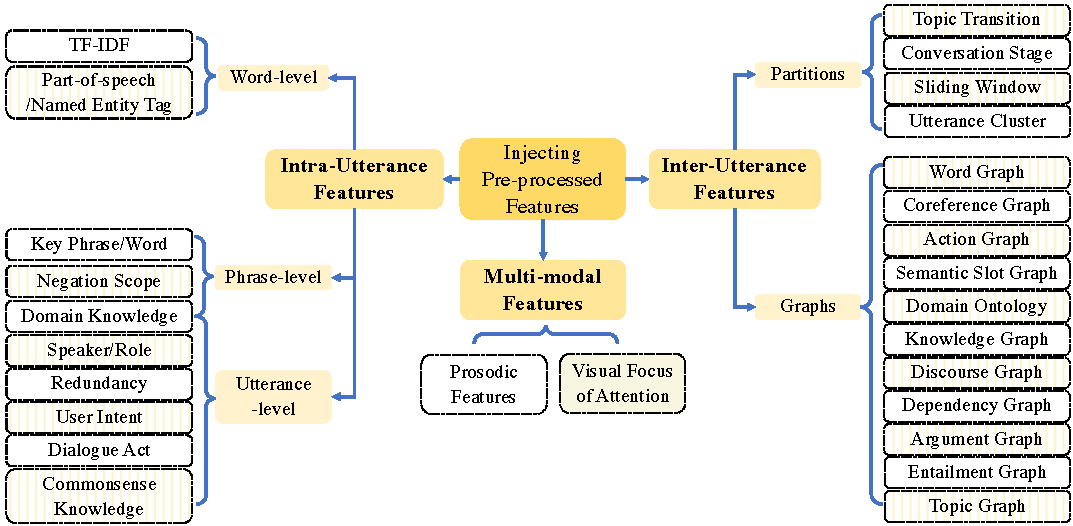
\includegraphics[scale=0.65]{fig/approach-feature.pdf}
	\caption{A summary of all features.}
	\label{fig:app-feature}
\end{figure}
The above features are summarized in 
Fig.~\ref{fig:app-feature} and mainly {injected into vanilla models} 
in three ways: 

\begin{itemize}
\item \textbf{Manipulating the input and output} by adding annotations or data reformulation. The former one adds additional tokens to the dialogue or summary to highlight the features, such as topic transition marks in the dialogue~\cite{chen2020multi} and key phrase prefixes of the summary~\cite{wu2021controllable}. This is suitable for features linearly buried in the texts. For the hierarchical or more complicated structures, researchers tend to reformulate the dialogue into different segments, especially for long dialogues~\cite{zhong2021qmsum,banerjee2015generating,shang2018unsupervised} or reordering utterances with graph features. For example,  \citet{fabbri2021convosumm} linearized the argument graph following a depth-first approach to fine-tune sequence-to-sequence models for summarization, and \citet{zhao2021todsum} linearized the dialogue states, i.e., slot-related labels, as a complement to $D$ with a bi-encoder model.



\item \textbf{Modifying the model architecture or hidden states} for learning inductive bias on known features. Embedding layers are always modified for word-level or phrase-level features indicating the binary or multi-class classification properties, including the POS embeddings in~\cite{zhu2020end} and medical concept embedding in~\cite{joshi2020dr}. Modifications on self-attentions and cross-attentions are used to merge multiple features and are also preferable to graph features. For instance, \citet{chen2020multi} modified the cross-attention layer for balancing and fusing hidden states of two kinds of labeled input from double encoders. \citet{lei2021hierarchical} changed the self-attention layer in the encoder with two speaker-aware attentions to highlight the information flow within the same speaker or among speakers. Different graph neural layers~\cite{feng2021incorporating,liu2021coreference,chen2021structure} are also introduced for capturing graph features.


\item \textbf{Adding additional training targets} means that features are regarded as a supervision output during training under multi-task learning and are ignored during inference. For example, \citet{goo2018abstractive}, \citet{li2019keep}, \citet{kim2022mind} used an additional decoder for dialogue act labeling, topic segmenting and commonsense knowledge generation, respectively.
\citet{yuan2019scaffolds} incorporated domain features by formulating domain classification as a multi-label binary classification problem for the whole $D$. All of them use utterance-level features to learn better encoder representations, which will lead to a high-quality summary.

\end{itemize}

The advantages and disadvantages of injecting pre-processed features are as follows:
\begin{itemize}
    \item[\Checkmark] Injecting pre-processed features as the mainstream research direction for dialogue summarization significantly improves the results compared with the basic summarization model. Features including negation scope, speaker/role, coreference graph, action graph and semantic slot graph pay more attention to generating consistent summaries, while most of the other features help to select valuable information for summarization.
    \item[\Checkmark] Such explicitly incorporated features are more interpretable to humans and can be manipulated for more controllable summaries. Different features can be selected and combined to promote the model performance in specific application scenarios.
        \item[\Checkmark] Features collected by labelers on other dialogue understanding tasks capture the essence of these tasks and also establish connections with various aspects of dialogue analysis.  Therefore, leveraging such features is a good way to alleviate the human labeling burden.
	\item[\XSolidBrush] Features are not transferable in different scenarios and some features are not compatible with each other, thus feature engineering is shown to be important.
	\item[\XSolidBrush] Labelers trained with other datasets are always out-of-domain compared to the targeting dialogue summarization scenario. Hyper-parameters introduced in labeling algorithms with these labelers need try and error for the domain transfer. 
	\item[\XSolidBrush] Error propagation exists in these dialogue summarization approaches. Incorrect features hinder the understanding of dialogues and lead to poor summaries. 
\end{itemize}